\section{Vorhaben}
\label{sec:AnalyseAufgabenstellung}
Die Aufgabe, die sich das Projekt CKi stellt, ist die Wissenserweiterung des Entwicklers. Dabei wird ein Programm geschrieben, welches einzelnen handgeschriebenen Ziffern erkennen kann. Dies geschieht mittels KI. Dabei wird die KI komplett vom Entwickler geschrieben. Da keine modernen externen Grundlagen verwendet werden, wird das Produkt, das Programm, nicht die Geschwindigkeit einer modernen KI erreichen. Dies spielt jedoch keine Rolle, da dieses Projekt nicht wegen des Endprodukts durchgeführt wird.

\section{Zielgruppe}
\label{sec:AnalyseZielgruppe}
Das Projekt CKi ist als solches nicht ausgelegt einem realen Anwendungszweck zu entsprechen oder eine Lösung oder einen Lösungsansatz für einen solchen zu bieten. Diesbezüglich liegt der einzige Nutzen von CKi nicht in dessen Produkt, sondern nur im Wissensgewinn und Verständnisgewinn für den Entwickler in den Bereichen der künstlichen Intelligents oder genauer im Bereich des maschinellen Lernens mit einem \textit{Convolutional Neural Network}, der Realisation von Anwendungen mit C++ und dessen Möglichkeiten Hardware direkt in die programminternen Abläufe einzubinden. Somit richtet sich CKi nicht nach dem Grundsatz ein bestmöglich nutzbares Produkt zu sein, sondern lediglich nach dem grössten Wissensgewinn für den Entwickler. Nach diesem Grundsatz ist die resultierende Zielgruppe der Entwickler und vereint so mehrere Rollen des Projektes CKi in einer Person.

\section{Anforderungen}
\label{sec:AnalyseAnforderungen}

\subsection{Must-haves}
\label{sec:AnalyseMustHaveS}
Die Must-haves wurden aus dem Themenblatt, welches am 15.09.2023 bei Walter Schnyder eingereicht wurde, übernommen und mit weiterführenden Elaborationen versehen.

\begin{itemize}
	\item 
	\textbf{Rückgabe in Prozentwerten, die die Wahrscheinlichkeit der Übereinstimmung mit dem digitalen Gegenstück der handgeschriebenen Zahl abbilden.} „Welche Zahl wurde (vermutlich) aufgeschrieben?“
	\\
	\textbf{Erläuterung:}
	Da ein simples neuronales Netzwerk für maschinelles Lernen durch ein „Netz“ aus Knotenpunkten gebaut wird und jeder dieser Knotenpunkte, auch die Knotenpunkte, welche bei einem solchen neuralen Netzwerk als Endschnittstellen fungieren, einzeln berechnet werden, erhält man, bei Anwendungsfall von CKi, eine multiple Anzahl von Prozentzahlen, welche zur Interpretation des gelieferten Endergebnisses verwendet werden können. Diese Rückgabe der einzelnen Prozentwerte erfolgt zum Beginn über eine Konsolenausgabe. Diese wird später, wie in \ref{sec:AnalyseNiceToHaveS} („Nice-to-haves“) unter GUI erläutert, in ein grafisches Nutzerinterface integriert und zu diesem Zeitpunkt evtl. auch interpretiert (wobei die einzelnen Prozentwerte weiterhin einsichtig bleiben sollten).
	
	\item \textbf{funktionales neuronales Netzwerk (trainiert auf Zahlenwert)}
	\\
	\textbf{Erläuterung:}
	Ein CNN-Algorithmus oder auch Convolutional Neural Network wird beim maschinellen Lernen oft bei der Interpretation von Bildern genutzt. Dabei wird das Bild in kleinere Abschnitte unterteilt und „einzeln“ an den gehirnähnlich aufgebauten Algorithmus weitergegeben.
	\begin{figure}[H]
		\centering
		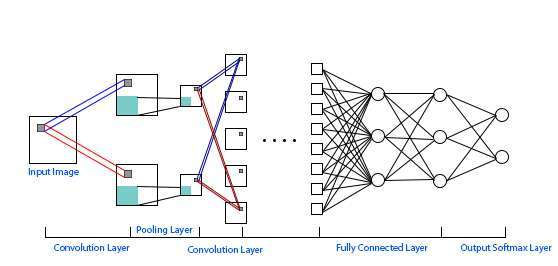
\includegraphics[scale=0.5]{CNN-model-with-several-convolution-and-pooling-layers-performed-alternately-combined.jpeg}
		%von https://www.researchgate.net/publication/309751512/figure/fig1/AS:503017750437888@1496940185276/CNN-model-with-several-convolution-and-pooling-layers-performed-alternately-combined.png
		\caption{CNN Model Aufbau Grafik von \href{https://www.researchgate.net/publication/309751512_Content-Aware_Convolutional_Neural_Network_for_Object_Recognition_Task}{researchgate.net}}
		\label{fig:AnalyseCNN-model-with-several-convolution-and-pooling-layers-performed-alternately-combined}
	\end{figure}
	Im Projekt CKi wird dieser wie im Themenblatt beschrieben mit Bildern von einzelnen handgeschriebenen Ziffern trainiert, dem MNIST-Datensatz.
	
	\item \textbf{Nutzer-Input | Nutzer darf eine Zahl zeichnen}
	\\
	\textbf{Erläuterung:}
	Ein solches CNN-Model zu erbauen und zu trainieren ist zwar die Grundlage für dieses Must-have, jedoch sollte das Produkt auch erprobbar sein. Diesbezüglich muss der Nutzer in der Lage sein, eine handschriftliche Ziffer an das neurale Netzwerk zu liefern. Hierbei ist die minimale Anforderung, dass der Nutzer in einer anderweitigen Applikation ein solches Bild erstellt hat und es nun interpretieren lassen kann. Wie in \ref{sec:AnalyseNiceToHaveS} („Nice-to-haves“) unter GUI beschrieben, wird diese Eingabemöglichkeit (eine Ziffer zu zeichnen oder eine schon vorhandene grafische Abbildung zu verwenden) in einem weiteren Entwicklungsschritt direkt in die zukünftige grafische Nutzeroberfläche der Applikation integriert.
	
\end{itemize}

\subsection{Nice-to-haves}
\label{sec:AnalyseNiceToHaveS}
Die Nice-to-haves wurden aus dem Themenblatt, welches am 15.09.2023 bei Walter Schnyder eingereicht wurde, übernommen und mit weiterführenden Elaborationen versehen. Zudem behalte ich mir als Verfasser dieses Dokumentes, als Entwickler des Projektes CKi und als Zielgruppe des Projektes CKi vor, diese Liste in gegebenen Fall zu erweitern.

\begin{itemize}
	\item \textbf{GUI}
	\\
	\textbf{Erläuterung:}
	Ein GUI (oder auch grafisches User-Interface) ist die grafische Nutzeroberfläche der Applikation. Da die Applikation primär dem Wissensgewinn gewidmet ist und dementsprechend nicht für den Nutzer optimiert wird, hat eine solche Erweiterung nur eine geringe Priorität. Diese Nutzeroberfläche wird selbst bei der Umsetzung in einer möglichst simplen Form gehalten. Dabei sollte es folgende Bestandteile beinhalten:
	\begin{itemize}
		\item Eine Möglichkeit für den Nutzer eine anderweitig gezeichnete Ziffer interpretieren zu lassen
		\item Eine Möglichkeit für den Nutzer eine Ziffer zu zeichnen.
		\item Eine (weiter-) interpretierte Ausgabe der Interpretation des CNN.
		\item Eine Ausgabe der nicht interpretierten Prozentwerte der Interpretation des CNN.
	\end{itemize}
	Bis zu dem Punkt, wo ein GUI realisiert wurde und in den Einsatz gestellt wird, sind nicht alle dieser Funktionen über die Konsole (das Interface zum Programm, welches vor dem GUI zum Einsatz kommt) verfügbar.
	
	\item \textbf{GPU als Berechnungsplattform nutzen}
	\\
	\textbf{Erläuterung:}
	Die CPU in einem Computer ist eine sehr „fokussierte“ Hardware. So kommt es dazu, dass diese immer nur einen einzelnen Prozess berechnen kann. Dies ist für ein neuronales Netzwerk, welches Hunderte oder Tausende Knotenpunkte hat und alle einzeln berechnet werden müssen, äusserst hinderlich. Eine dezidierte Grafikkarte, wenn vorhanden, kann diesem Geschwindigkeitsverlust nachhelfen, da eine solche GPU in der Lage ist, tausende Berechnungen gleichzeitig zu tätigen.
	Da im Projekt mit C++, einer Hardware-nahen Programmiersprache, gearbeitet wird, kann eine Anbindung an das Rechenpotential der GPU implementiert werden. Da dies jedoch ein äusserst schwieriger Prozess ist, sich diese Anbindung bei den unterschiedlichen Herstellern von GPUs unterscheiden kann und nicht notwendig ist, um ein funktionierendes CNN zu erstellen, wurde diese Optimierung als nicht notwendig eingestuft.
\end{itemize}

\subsection{Use Cases}
\label{sec:AnalyseUseCases}
Die hier aufgelisteten Use Cases entsprechen den Use Cases nach den Must-haves und sind diesbezüglich ohne die grafische Nutzeroberfläche. Dies kann dazu führen, dass ein endgültiges Produkt nicht mehr kohärent zu den Use Cases steht. Im Allgemeinen sollte aber selbst eine solche Inkohärenz nicht in extremer Weise auftreten, da die Bedienung der Applikation als Konsole als auch als grafische Oberfläche in ähnlicher Weise auftreten sollte.
\begin{enumerate}
	\item \textbf{Prediction}
		\begin{itemize}
			\item \textbf{Akteur:} Nutzer, CNN
			\item \textbf{Ablauf:} Siehe Ablaufdiagramm \ref{sec:AnalyseInterpretation} („Interpretation“).
			\item \textbf{Nachbedingungen:} Der Nutzer sollte in der Konsole eine Auflistung aller möglichen Ziffern (0–9) und deren entsprechende Wahrscheinlichkeit sehen. Zudem kann der Nutzer auch die kongruierende Zahl mit der höchsten Wahrscheinlichkeit auf einer speziellen Zeile in der Konsole ablesen.
			\item \textbf{Ausnahmen:} Bei der Interpretation von benutzereigenen Abbildungen kann es zu multiplexen Fehlern kommen. Diese reichen von falscher Dateikodierung zu falscher Auflösung. Aufgrund dieser mannigfaltigen Möglichkeiten zu Fehlern können diese nicht alle hier erläutert werden.
			\item \textbf{Anmerkungen:} Offiziell ist zwar „Training“ keine Vorbedingung von „Testen“, jedoch macht die Anwendung der Applikation keinen Sinn, wenn man nicht erwarten kann, dass man ein realistisches oder sinnvolles Ergebnis erhält.
		\end{itemize}
	\item \textbf{Training}
	\begin{itemize}
		\item \textbf{Akteur:} Nutzer, CNN
		\item \textbf{Ablauf:} Siehe Ablaufdiagramm \ref{sec:AnalyseTraining} („Training“).
		\item \textbf{Nachbedingungen:} Der Nutzer erhält nach der Beendigung der Schulung des CNN-Models eine kurze Benachrichtigung, dass das Training abgeschlossen ist. Zudem erhält der Nutzer nach jedem einzelnen Datensatz den Output, dass nun x von y Datensätzen bearbeitet wurden (kann auch als Lade-Balken oder Ähnliches (Ladetext) implementiert werden).
		\item \textbf{Ausnahmen:} Hierbei kann es zu zwei Fehlern kommen. Dabei handelt es sich um Fehler bei den Datensätzen. Der eine Fehler ergibt sich aus der Möglichkeit, dass CKi die entsprechende Datei aus befindlichen Gründen nicht öffnen kann.
Der andere Fehler ergibt sich, wenn der Datensatz nicht dem Standard der MNIST-Datensätze im UByte-Format entspricht.
\\
Natürlich können auch andere Fehler eintreten, diese können nicht zu diesem Zeitpunkt abgeschätzt werden.
	\end{itemize}
	\item \textbf{Testing}
	\begin{itemize}
		\item \textbf{Akteur:} Nutzer, CNN
		\item \textbf{Ablauf:} Siehe Ablaufdiagramm \ref{sec:AnalyseTesten} („Testen“).
		\item \textbf{Nachbedingungen:} Der Nutzer erhält eine Benachrichtigung, dass x von y Datensätzen bearbeitet wurden (kann auch als Lade-Balken oder Ähnliches (Ladetext) implementiert werden). Nach Beendigung erhält der Nutzer die Mitteilung, dass das Testen abgeschlossen ist und einen Prozentwert mit der Genauigkeit des Netzwerkes.
		\item \textbf{Ausnahmen:} Hierbei kann es zu zwei Fehlern kommen. Dabei handelt es sich um Fehler bei den Datensätzen. Der eine Fehler ergibt sich aus der Möglichkeit, dass CKi die entsprechende Datei aus befindlichen Gründen nicht öffnen kann.
Der andere Fehler ergibt sich, wenn der Datensatz nicht dem Standard der MNIST-Datensätze im UByte-Format entspricht.
Natürlich können auch andere Fehler eintreten, diese können nicht zu diesem Zeitpunkt abgeschätzt werden.
		\item \textbf{Anmerkungen:} Bei den Testdaten würde es evtl. Sinn ergeben, die einzelnen Konsolen Outputs auch in einer CSV-Datei festzuhalten, wobei dies mit Pipes in der Konsole dem Nutzer bereits offensteht. Offiziell ist zwar „Training“ keine Vorbedingung von „Testen“, jedoch ergibt das Testen nur begrenzt Sinn, wenn es noch nichts gibt, was sich zu testen lohnt.
	\end{itemize}
\end{enumerate}

\subsection{Use Case Diagramme}
\label{sec:AnalyseUseCaseDiagramme}
\begin{figure}[H]
	\centering
	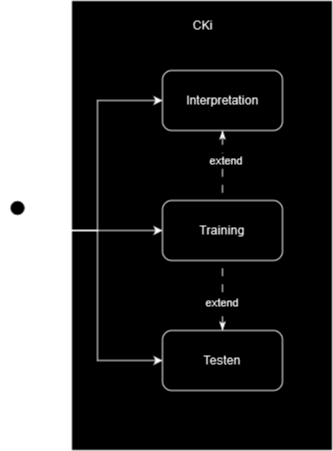
\includegraphics[height=0.35\paperheight]{usecase.png}
	\caption{Use-Case-Diagramm}
	\label{fig:analyseusecase}
\end{figure}

\subsection{Ablaufdiagramme}
\label{sec:AnalyseAblaufdiagramme}

\subsubsection{Interpretation}
\label{sec:AnalyseInterpretation}
\begin{figure}[H]
	\centering
	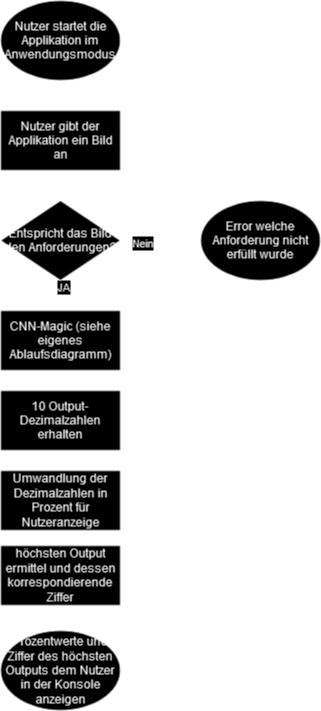
\includegraphics[height=0.5\paperheight]{ablauf-interpretation.png}
	\caption{Ablaufdiagramm für die Interpretation von Nutzer-gelieferten Einzelbildern}
	\label{fig:analyseablauf-interpretation}
\end{figure}


\subsubsection{Training}
\label{sec:AnalyseTraining}
\begin{figure}[H]
	\centering
	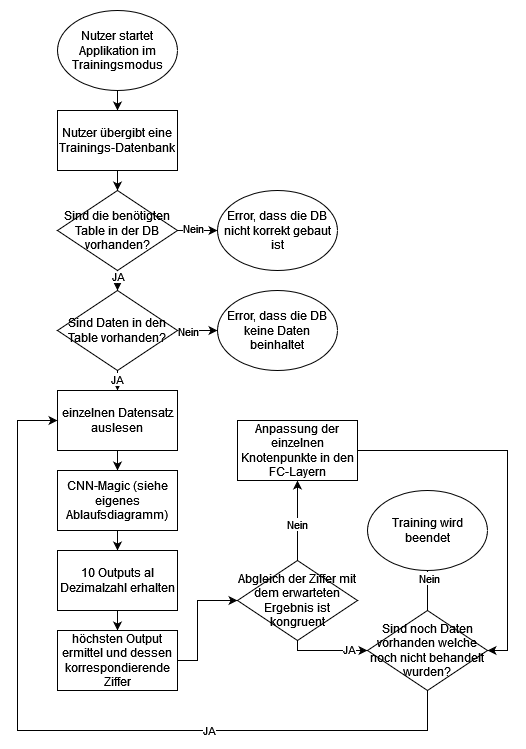
\includegraphics[height=0.65\paperheight]{ablauf-training.png}
	\caption{Ablaufdiagramm vom Training des CNN}
	\label{fig:analyseablauf-training}
\end{figure}


\subsubsection{Testen}
\label{sec:AnalyseTesten}
\begin{figure}[H]
	\centering
	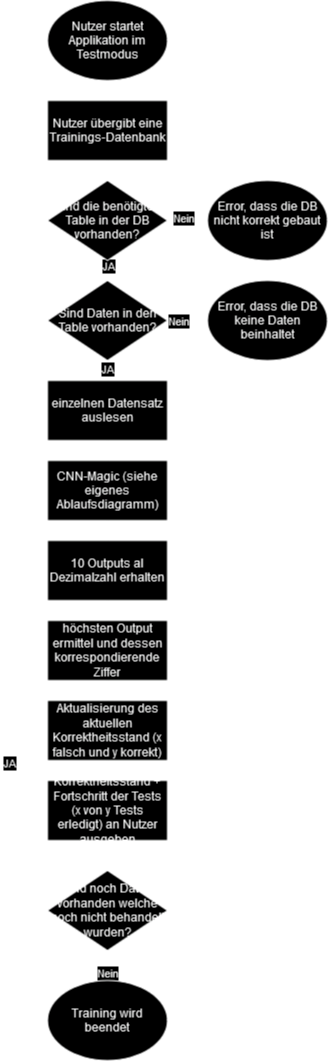
\includegraphics[height=0.65\paperheight]{ablauf-testen.png}
	\caption{Ablaufdiagramm von einem Test des CNN}
	\label{fig:analyseablauf-testen}
\end{figure}


\subsubsection{CNN-Magie}
\label{sec:AnalyseCNN-Magic}
\begin{figure}[H]
	\centering
	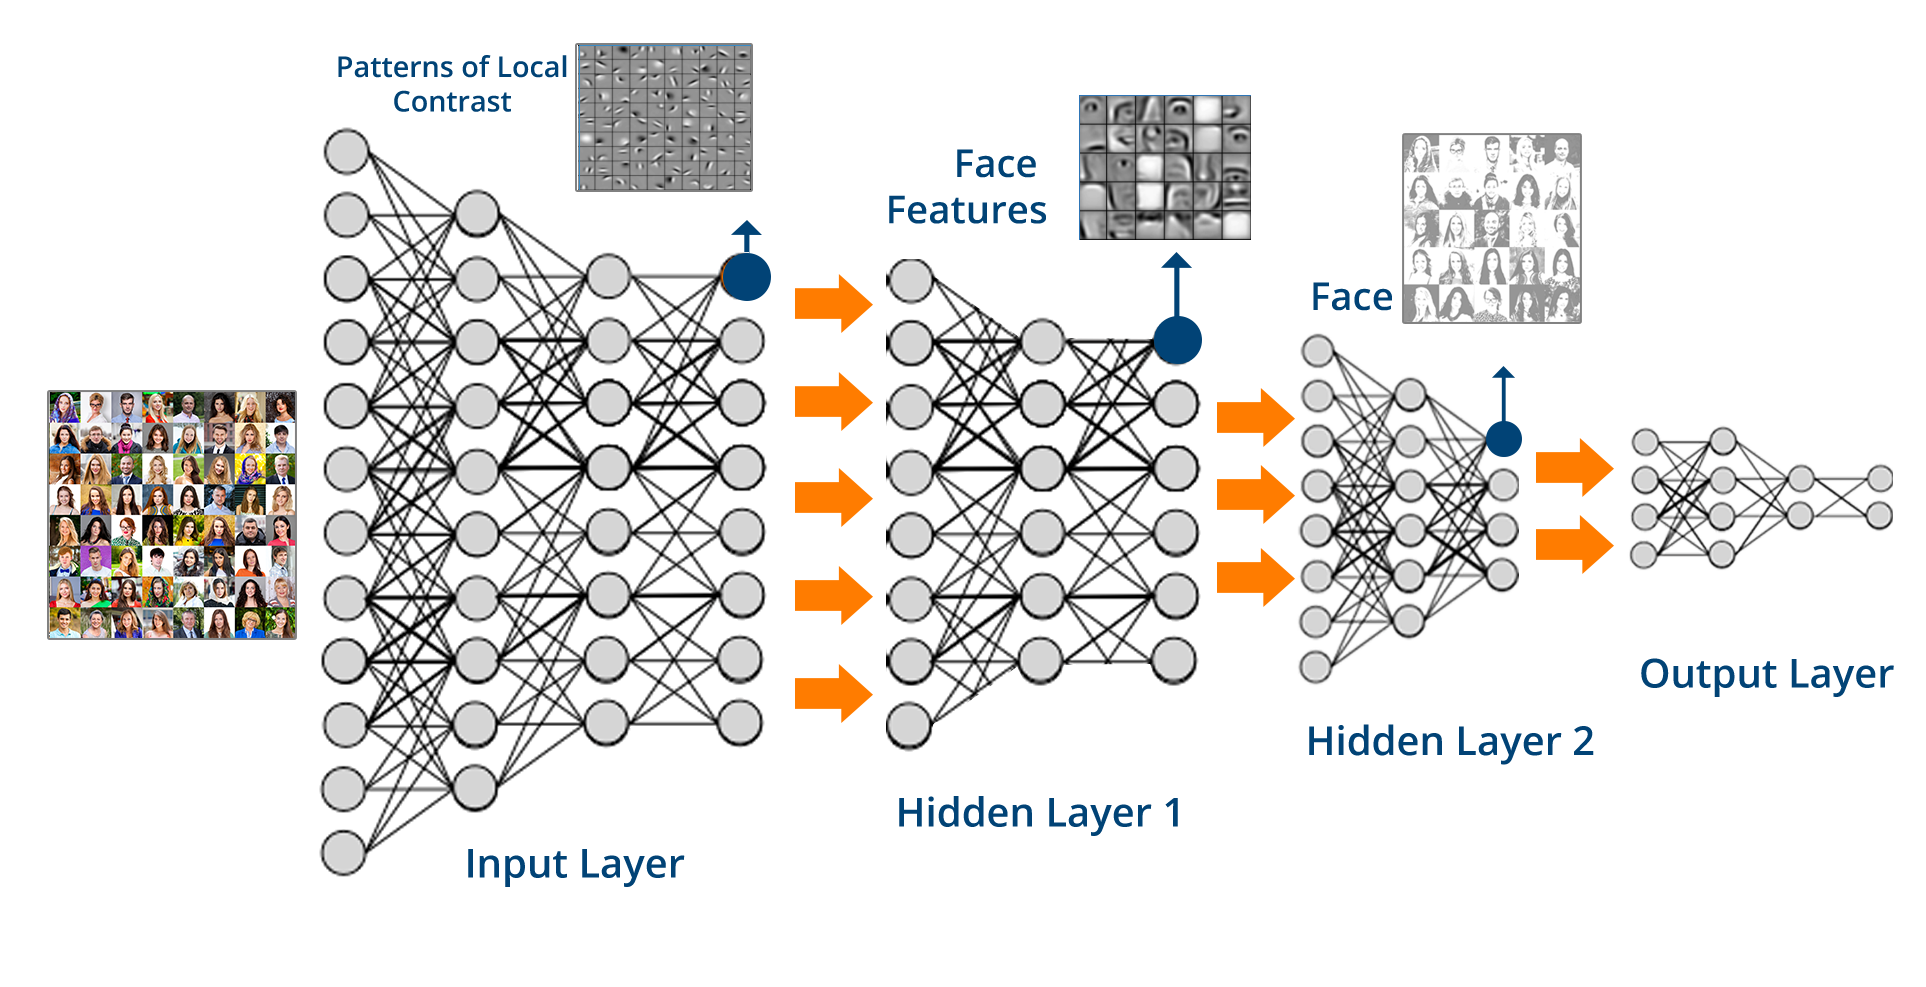
\includegraphics[width=\linewidth]{1RXJ6tAmfN1AYLQr7p48L7w-631173908.png}
	\caption{Visuelle Darstellung der Funktionsweise eines CNN von \href{https://blog.goodaudience.com/cnn-for-rnns-a-gentle-approach-to-use-cnns-for-nlp-53ab80768d43}{blog.goodaudience.com}}
	\label{fig:analyse1RXJ6tAmfN1AYLQr7p48L7w-631173908}
\end{figure}

\section{Umsetzung}
\label{sec:AnalyseUmsetzung}
Wie im Themenblatt vom 15.09.2023 wird für die Umsetzung reines C++ verwendet.

\subsection{Entwicklungsumgebung}
\label{sec:AnalyseEntwicklungsumgebung}
Bei der Entwicklungsumgebung wird das JetBrains Produkt \textbf{CLion} zum Einsatz kommen. Dieses beinhaltet alle benötigten Funktionalitäten, die bei der Entwicklung des Produktes nötig sind. Gegebenen Falles könnte noch \textbf{SQLite Browser} zur Verwendung kommen, da dieses ein besseres (und für den Entwickler ein gewohntes) Interface zur Handhabung von lokalen Datenbanken bietet. (Dieses Produkt kam nicht zum Einsatz, da keine Datenbank verwendet wurde.) Für die Version Control des Projektes wird lokal \textbf{Git} verwendet und zur Sicherung in der Cloud wird sowohl \textbf{GitHub} als auch \textbf{GitLab} verwendet. Die Entwicklungsumgebung mit IDE und Version Control wird primär auf dem Betriebssystem Windows verwendet. Es kann jedoch nicht garantiert sein, dass die Entwicklung nicht teilweise unter einer Distribution von Linux ablaufen wird. Hierbei sollten (evtl. abgesehen von der GUI) keine Kompatibilitätsprobleme auftreten. 
\subsubsection{Auflistung Versionen}
\label{sec:AnalyseDevEnvAuflistung}
\begin{itemize}
	\item JetBrains Toolbox 2.1.1.18388, Windows 11, x64
	\item CLion (von JetBrains Toolbox) 2023.2.2
	\item Git 2.39.2.windows.1
	\item CMake 3.27.7
	\item GCC 13.2.0
	\item MiKTeX 23.10
	\item TeXnicCenter 2.02
\end{itemize}

\subsection{CNN}
\label{sec:AnalyseCNN}
\subsubsection{Grundlagen}
\label{sec:AnalyseGrundlagen}
Der Kern des CNN lässt sich in drei unterschiedliche Arten von Schichten aufteilen. Zusätzlich gibt es noch zwei zusätzliche „Hilfs-“Schichten, welche für die Ein- und Ausgaben zuständig sind. 
Die \textit{Eingabeschicht} ist eine dieser zwei erwähnten Schichten. Diese akzeptiert im Falle von CKi jeweils ein Bild von speziell definierten Grössen und nimmt jeden Pixel als Graustufen (Dies ist entscheidend, weil so der Farbwert des Pixels von drei zwei Byte grossen Zahlen zu nur einer zwei Byte grossen Zahl reduziert wird.) als Eingabe entgegen. 
Auf die Eingabeschicht folgt die \textit{Convolutional Layers} oder auch \textit{Faltungsschichten}. Diese Faltungsschichten sind einer der Schlüsselbestandteile eines CNN. Die Convolutional Layer dienen dazu, bestimmte Merkmale und Schlüsselelemente aus dem Bild zu extrahieren. Hierbei wird bei jedem der Convolutional Layer eine 
mathematische Faltungsoperationen durchführt. 
Nach den Faltungsschichten kommen die simplen \textit{Pooling-Schichten}. Bei einer Pooling-Schicht wird die Dimension eines Bildes reduziert (Downsampling). Dies kann durch zwei Arten geschehen, entweder durch Max-Pooling, dabei wird aus einer Liste von Werten nur der höchste übermittelt oder durch Durchschnitts-Pooling, wobei der Durchschnitt dieser Liste berechnet und übermittelt wird. Durch diese Datenreduktion wird Rechenleistung gespart und so das Ergebnis schneller und stabiler geliefert. 
Vor der Ausgabeschicht gibt es noch die \textit{FC Layers} oder auch \textit{Vollständig verknüpfte Schichten} (\textit{Hidden Layers}). Bei diesen ist jeder Knotenpunkt mit jedem Knotenpunkt in der nächsten Schicht verbunden. Dies ist das Herz des gesamten Models. Dabei wird in jedem Knotenpunkt ein neuer Wert berechnet, um in der letzten Schicht, der \textit{Ausgabeschicht} diese in Wahrscheinlichkeit zu „konvertieren“.\footnote{vgl. Pathak, 2023; IBM, 2021; Saha, 2018; 3Blue1Brown, 2017}

\subsubsection{Implementation}
\label{sec:AnalyseImplementation}
Bei der Implementation eines neuronalen Netzwerkes wurde für CKi der Entschluss getroffen, eine C++-Klasse für jede benötigte Art von Komponente, die die Applikation benötigt, zu kreieren. Konkret bedeutet dies, dass eine Klasse für das Neuron, eine für den Layer und eine für das Netzwerk entstehen muss. Dabei werden die Klassen aufeinander aufgebaut; ein Netzwerk hat multiple Layer, ein Layer hat multiple Neuronen. Dieses Netzwerk wird danach in die Main-Funktion, den Programmeinstieg, integriert. Dies erleichtert es, in einem späteren Schritt die grosse Umstellung von einer Konsolen-Anwendung hin zu einer grafisch basierten Anwendung (auch wenn immer noch grosse Teile der Main-Klasse ausgetauscht werden müssen). Für die Speicherung der Berechnungswerte für die FC-Layer ist die Abwägung zu treffen, ob es sinnvoll ist, diese in einer lokalen Datenbank zu speichern oder in eine konkret hierfür entworfene Datei zu schreiben.

\subsection{Testdaten}
\label{sec:AnalyseTestdaten}
Die Testdaten für CKi können in unzähliger Ausführung auf \href{https://www.kaggle.com/}{Kaggle} gefunden werden. Es wird jedoch der Standard von \url{http://yann.lecun.com/exdb/mnist/} verwendet.

\subsubsection{Speicherung}
\label{sec:AnalyseSpeicherung}
Im gegebenen Fall würde es für die Schulung, des CNN, Sinn ergeben, die einzelnen Bilder nicht über Ordner- oder Archivstrukturen zu speichern, sondern in eine oder mehrere lokale Datenbanken abzuspeichern.
\\
Im Falle von \url{http://yann.lecun.com/exdb/mnist/} ist dies jedoch nicht notwendig, da diese im UByte-Format vorliegen, wie in \ref{sec:DesignUByte} beschrieben.

\section{Abwägung des Nutzens und der Alternativen}
\label{sec:AnalyseNutzwertanalyseDerLösungsvarianten}
\subsection{Alternativen}
\label{sec:AnalyseAlternativen}
Die möglichen Alternativen zu einer kompletten Realisation eines CNN oder eines neuronalen Netzwerks in C++ ohne Bibliotheken oder Frameworks für neuronale Netze sind endlos. 
Wenn gleich man bereits bestehende Produkte begutachtet, wird man auf GitHub schnell fündig. Bei einer Suche auf GitHub mit dem Query „mnist digit recogniser“ findet man nach Stand 20.10.2023 02:13 178 Repositorien (je eines in C, C++, C\#, Rust, drei in Java + Kotlin und 53 in Python).
Auch unter dem Beschluss, dass man das CNN selbst bauen wolle, würde man für jede beliebige Sprache eine Bibliothek oder Framework finden, das einem diese Aufgabe erleichtern würde.

\subsection{Kosten}
\label{sec:AnalyseKosten}
Bezüglich der Kosten kann das Projekt CKi nicht mit den Alternativen mithalten. C++ ist keine Sprache, in welcher man schnell ein Produkt hervorbringt. Dies belegen etliche Studien und Artikel (
\href{https://www.cs.bsu.edu/homepages/dmz/cs697/langtbl.htm}{Programming Languages Table}, 
\href{https://citeseerx.ist.psu.edu/viewdoc/download?doi=10.1.1.113.1831&rep=rep1&type=pdf}{An Empirical Comparison of Seven Programming Languages},
\href{https://haslab.github.io/SAFER/scp21.pdf}{Programming Languages by Energy Efficiency}, 
\href{https://stackoverflow.com/questions/1894453/development-time-in-various-languages}{Development time in various languages}).
Zu dem, dass keine dezidierten Bibliotheken für maschinelles Lernen zum Einsatz kommen, erhöht den Entwicklungsaufwand, Zeitaufwand und so die Kosten.
Wenn man die Stundenzahl aus der Planung mit einem Stundensatz von 50 CHF quantifizieren, käme man auf einen gesamten Kostenaufwand von 8'600.- + Lizenzkosten. Zuzüglich kämen noch Hardware Anschaffungen für die Entwicklung hinzu, diese können jedoch im Falle vom Projekt CKi vernachlässigt werden.  

\begin{xltabular}{\linewidth}{|X|c|r|}
	\hline
	Senior Developer & 2h & 100.00 Fr.
	\\\hline
	Junior Developer & 89h & 4'450.00 Fr.
	\\\hline
	Projektleitung & 39h & 1'950.00 Fr.
	\\\hline
	Hardware & - & 0.00 Fr.
	\\\hline
	Software & Lizenz & 827.00 Fr.
	\\\hline\hline
	Möglicher Zusatz-Entwicklungskosten  & 42h & 2'100.00 Fr.
	\\\hline\hline
	Total &  & 9'427.00 Fr.
	\\\hline
\end{xltabular}
\label{tab:AnalyseKostenTable}
\addcontentsline{lot}{table}{\protect\numberline{\thetable}Kostenanalyse}

\subsection{Nutzen}
\label{sec:AnalyseNutzen}
Wie bereits im Abschnitt Zielgruppe \ref{sec:AnalyseZielgruppe} erwähnt, ist dieses Produkt auf den Wissensgewinn ausgerichtet und nicht auf das Produkt selbst. Dementsprechend ist in der geplanten Umsetzung des Projektes CKi der maximale Nutzen gewährleistet. Leider lässt sich dieser Nutzen nicht/schlecht quantifizieren.

\subsection{Effizienz}
\label{sec:AnalyseEffektivität}
Der Vergleich in Effizienz der Anwendung, der aus dem Projekt CKi resultiert und den professionell entwickelten Bibliotheken in Python, etc., wird CKi selbst mit GPU-Berechnung und dem Geschwindigkeitsvorteil von C++ gegen diese Bibliotheken in Bezug auf Run-Time-Length verlieren.

\subsection{Vergleich}
\label{sec:AnalyseVergleich}

\begin{xltabular}{\linewidth}{|X|X||X|X|}
	\hline
	\multicolumn{2}{|c||}{Bestehendes Produkt} & \multicolumn{2}{c|}{Eigene Kreation}
	\\\hline
	Sektion & Kosten & Sektion & Kosten
	\\\hline
	Anschaffungskosten & 0.- Fr.  & Kreation & 8'600.- Fr.
	\\\hline
	Wiederholende Kosten & 0.- Fr. & wiederholende Kosten & 0.- Fr.
	\\\hline\hline
	Absolut & 0.- Fr. & absolut & 8'600.- Fr.
	\\\hline
\end{xltabular}
\label{tab:AnalyseVergleichTable}
\addcontentsline{lot}{table}{\protect\numberline{\thetable}Vergleich bestehendes Produkt gegen eigene Kreation}
\noindent Eine kurze Zusammenfassung der Kosten-Nutzen-Analyse zeigt den Zustand von CKi.
\\
Es werden Kosten für die Arbeitszeit von 8'600 CHF anfallen. Die Effektivität ist niedriger, als wenn dasselbe Produkt mit einer vorhandenen Bibliothek geschrieben werden würde (und die Entwicklungsdauer wäre ebenfalls geringer). Des Weiteren gibt es unzählige kostenlose Alternativen, die es nur zu verwenden gilt.
\\
Der Nutzen des Endproduktes ist nichtig, da dieses nie zur wirklichen Anwendung kommen wird.

\subsection{Nutzwertanalyse}
\label{sec:AnalyseNutzwerkanalyse}
Bei der Nutzwertanalyse werden unterschiedliche Alternativen systematisch und statistisch nach gewissen Kategorien verglichen. Konkret werden hier unterschiedliche Möglichkeiten der Implementierung miteinander verglichen, dabei wird eine Punkteskala von eins bis zehn verwendet. Wichtig bei der Auflistung ist es, dass eine höhere Punktzahl nicht bedeutet, wie hoch diese Kategorie ist. Eine Entwicklungsdauer von 10 bedeutet nicht, dass diese besonders lang ist, sondern dass diese Option im Bereich Entwicklungsdauer zehn Punkte erhalten hat (also besonders schnell zum implementieren ist).

\begin{xltabular}{\linewidth}{|l|l||c|c||c|c|}
	\hline
	\multicolumn{2}{|X||}{Kriterien} & \multicolumn{2}{X||}{Python mit TensorFlow} & \multicolumn{2}{X|}{C++}\\\hline Entwicklungsdauer & 10 \% & 10 & 1 & 2 & 0.2
	\\\hline
	Komplexität & 15 \% & 10 & 1.5 & 4 & 0.6
	\\\hline
	Sprachkenntnisse & 10 \% & 3 & 0.3 & 4 & 0.4
	\\\hline
	Frust & 10 \% & 5 & 0.5 & 7 & 0.7
	\\\hline
	Typisierung & 5 \% & 1 & 0.05 & 9 & 0.45
	\\\hline
	Run-Time-Length & 10 \% & 10 & 1 & 9 & 0.9
	\\\hline
	Testing & 5 \% & 6 & 0.3 & 7 & 0.35
	\\\hline
	Objektorientiert & 5 \% & 5 & 0.25 & 9 & 0.45
	\\\hline
	Wissensgewinn & 30 \% & 2 & 0.6 & 10 & 3
	\\\hline\hline
	Total & 100 \% & 52 & 5.5 & \hl{61} & \hl{7.05}
	\\\hline
\end{xltabular}
\addcontentsline{lot}{table}{\protect\numberline{\thetable}Nutzwertanalyse}

\label{tab:AnalyseNutzwertanalyse}


